\chapter{Lecture 8 - Geospatial data and Best Practice}
\subsubsection{Recap \emph{Geometry} dataset type}
The geometry dataset type specifies information about the shape of items with explicit spatial positions. The items can be represented as points, lines, or surfaces. This type of data may not have any attributes. \par
The given spatial position is an attribute of primary importance; the central tasks often revolve around understanding spatial relationships. A sensible visual encoding choice is to use the provided spatial position as the substrate for the visual layout, rather than to visually encode other attributes using the spatial position channel.

\section{Choropleth map}
A choropleth map shows regions as area marks, and a quantitative attribute is encoded as color over regions; also, texture can be used as a channel. Usually employed for showing how a quantity is distributed across geographical areas. \par
It is a good choice for an overview rather than for an accurate comparison, because of the use of the color channel for quantitative data. \par
One of the main risks of this visualization is the confusion of geographic area and population with data values, e.g., showing where people live instead of actual data. \par
The major design choices for a choropleth map are: how to construct the color map and what region boundaries to use, i.e., spatial aggregation (should the region granularity be a country, a state, or a city?). \par
Overall, the choropleth map is useful to display how data is distributed over geographical regions. The ideal situation would be when regions have approximately the same size, so always ask yourself whether the data should be normalized or not. An important point is to pay attention to the choice of the color map according to the semantics of the data (is it sequential or diverging?) and to the number of bins. It can be an easy tool for conveying messages, thanks to the familiar and natural representation of the spatial data. However, be careful to not to pass the wrong message, and how the data is presented, it is easy to communicate the area (bin size) rather than the actual data, also the strong dependence on color might make it confusing. 

\subsubsection{Recap: Choropleth map}
\begin{tabularx}{0.8\textwidth} { 
  | >{\raggedright\arraybackslash}l 
  | >{\raggedright\arraybackslash}X | }
    \hline
    Data (What) & Geographic geometry data using a table with one quantitative attribute per region \\
    \hline
    Encode (How) & The use of given geometry for area mark boundaries to represent space, and the use of sequential segmented color map \\
    \hline
\end{tabularx}

\begin{figure}[hbtp]
    \centering
    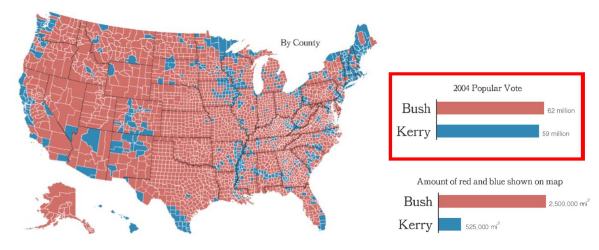
\includegraphics[width=0.5\linewidth]{imgs/lecture8/8.1 choropleth map.png}
    \caption{Choropleth map and message conveying ability}
    \label{fig:8.1}
\end{figure}

\section{Symbol map}
A symbol map, which can be a disk, a square, or a shape, is placed at a point and scaled such that its area is proportional to the quantity associated with the point. We can use area, shape, and color as channels. Unlike a choropleth map, a symbol map avoids confusing geographic areas with data values. One can even use graphs/charts/complex glyphs as symbols, even encoding multiple attributes. \par
A symbol map can be intuitive and easy to understand, they solve the issue of region dimension vs the value of the visualized attribute, because the symbol dimension is proportional to the data value and not to the region dimension. However, when encoding the data using a symbol map, one should try to avoid complex symbols, for they can be harder to understand; and the symbols' placement can be an issue: some symbols can overlap and hide other symbols or even region boundaries.

\begin{figure}[htbp]
    \centering
    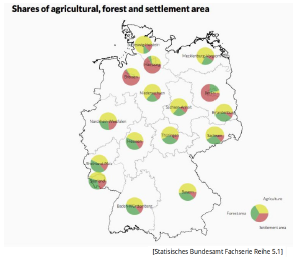
\includegraphics[width=0.3\linewidth]{imgs/lecture8/8.2 symbol map.png}
    \caption{Symbol map}
    \label{fig:8.2}
\end{figure}

\section{Dot density map}
A dot density map typically uses points as marks, and points are positioned over a map, where each dot represents a given constant quantity of items; all dots are equal, it is their quantity and distribution that gives information. \par
A dot density map is easy and intuitive, which mitigates the confusion between region areas and displayed values. But an accurate estimate can be difficult to make, due to the overlap of information and the quantity of dots. Sometimes, the normalization may be needed (for example, 1 dot = number cases / 1000 people).

\begin{figure}
    \centering
    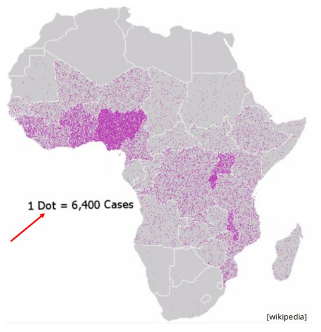
\includegraphics[width=0.3\linewidth]{imgs/lecture8/8.3 dot density map.png}
    \caption{Dot density map}
    \label{fig:8.3}
\end{figure}

\section{Contiguous cartogram}
It is a particular representation of the data where the geographic position and boundaries among regions are preserved, while dimensions are distorted according to a quantitative attribute. The aim is to preserve as much as possible the original position, shape, and boundary, and minimize distortion.

\begin{figure}[htbp]
    \centering
    
    \begin{subfigure}{0.45\textwidth}
        \centering
        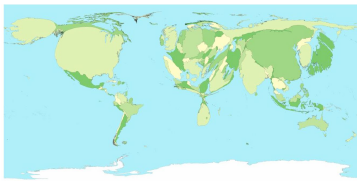
\includegraphics[width=0.6\linewidth]{imgs/lecture8/8.4 contiguous cartogram.png}
        \caption{Contiguous cartogram}
        \label{fig:8.4a}
    \end{subfigure}
    \hfill
    \begin{subfigure}{0.45\textwidth}
        \centering
        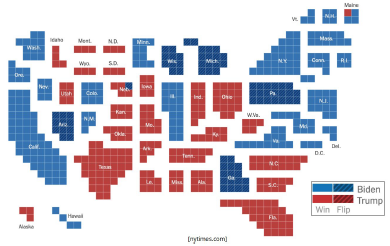
\includegraphics[width=0.6\linewidth]{imgs/lecture8/8.5 grid cartogram.png}
        \caption{Grid variation}
        \label{fig:8.4b}
    \end{subfigure}

    \caption{Contiguous cartogram and its grid variant}
    \label{fig:8.4}
\end{figure}

\section{Best practice - ten rules}
There are some recommended best practices that one should keep in mind when choosing a visualization tool. The ten rules are: best channel first; ensure accuracy and transparency; no unjustified 2D; no unjustified 3D; eyes beat memory; overview first, zoom and filter, details on demand; responsiveness is required; pay attention to color; function first, form next; self-contained visualizations

\subsection{Best channels first}
Recall the \textit{effectiveness principle}: the relevance of information displayed should match the effectiveness of the channel. Meaning that the relevant information should be prioritized, then encoded with the most effective/accurate channels. \par
We have seen channel rankings; to follow this rule means to use the highest-ranked channels for the most important attributes, and the other channels for the remaining, secondary attributes.

\subsection{Ensure accuracy and transparency}
Recall the expressiveness principle: the visual representation should represent all of, and only, the relationships that exist in the data. This implies that information that is not present in the data should not be visualized. It is also important to not to convey misleading information while paying attention to axis starting values and scale, and align data when possible for accurate comparisons, and more.

\subsection{No unjustified 3D}
Misconception: \textit{if two dimensions are good, then three dimensions must be better}. \par
There are many difficulties in visually encoding information with the third spatial dimension, depth. 3D visualization is justified only when the user's task involves shape understanding of inherently three-dimensional structures; usually, these inherently spatial data are scientific visualization and computer graphics, where the use of 3D is fundamentally required for understanding the three-dimensional geometric structure of objects or scenes. In all other contexts, the use of 3D needs to be carefully justified. \par

\begin{figure}[htbp]
    \centering
    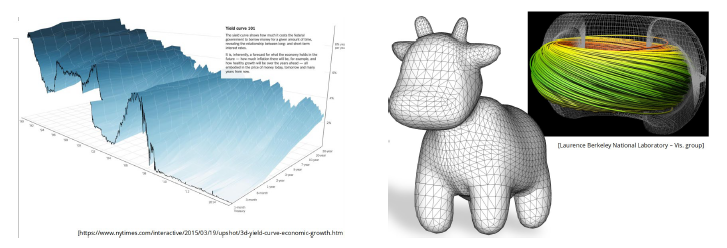
\includegraphics[width=0.5\linewidth]{imgs/lecture8/8.6 justified 3d.png}
    \caption{Justified 3D use cases}
    \label{fig:8.5}
\end{figure}

One of the main issues is occlusion, where some objects cannot be seen because they are hidden behind others. The overarching problem with occlusion in the context of visual encoding is that presumably important information is hidden (the occluded detail might even be critical), and discovering hidden details via navigation has a time cost.\par
In visually encoding abstract data, perspective is another very bad thing. Perspective distortion is one of the main dangers of depth because the power of the plane is lost; it completely interferes with visual encoding that uses the planar spatial position channels and the size channel, e.g., it is more difficult to judge and compare bar heights in a 3D bar chart than in multiple horizontally aligned 2D bar charts. \par
Another problem with the use of 3D is dramatically impaired text legibility. Text fonts have been very carefully designed for maximum legibility when rendered on the grid of pixels that makes up a 2D display. Text tilted in any way off the image plane typically becomes jaggy.

\begin{figure}[htbp]
    \centering
    
    \begin{subfigure}{0.45\textwidth}
        \centering
        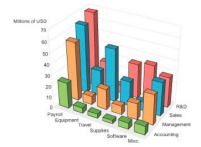
\includegraphics[width=0.6\linewidth]{imgs/lecture8/8.7 unsjustified 3d.png}
        \caption{Perspective issue}
        \label{fig:8.6a}
    \end{subfigure}
    \hfill
    \begin{subfigure}{0.45\textwidth}
        \centering
        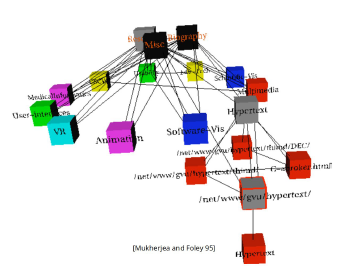
\includegraphics[width=0.6\linewidth]{imgs/lecture8/8.8 unjustified 3d.png}
        \caption{Text legibility issue}
        \label{fig:8.6b}
    \end{subfigure}

    \caption{Unjustified 3D use cases}
    \label{fig:8.6}
\end{figure}

\subsection{No unjustified 2D}
Laying out data in a 2D space should be explicitly justified, compared with the alternative of simply showing the data with a 1D list.

\subsection{Eyes beat memory}
Using our eyes to switch between different views that are visible simultaneously has a much lower cognitive load than consulting our memory to compare a current view with what was seen before. \par
The phenomenon of change blindness is that we fail to notice even quite drastic changes if our attention is directed elsewhere. Although we are very sensitive to changes at the focus of our attention, we are surprisingly blind to changes when our attention is not engaged. The difficulty of tracking complex and widespread changes across multi-frame animations is one of the implications of change blindness for visualization.\par
In simpler words, seeing lasts longer than remembering, but distraction prevents us from noticing changes.

\subsection{Overview first, zoom and filter, details on demand}
This is a visualization idiom that provides an overview is intended to give the user a broad awareness of the entire information space with the goal of summarizing. An overview helps the users to find regions where further investigation in more detail might be productive. An overview is often shown at the beginning of the exploration process to guide users in choosing where to drill down to inspect in more detail.

\subsection{Responsiveness is required}
The latency of interaction, namely, how much time it takes for the system to respond to the user action, matters immensely for interaction design. Human reaction to phenomena is best modeled in terms of a series of discrete categories, with a different time constant associated with each one. A system will fell responsive if these latency classes are taken into account by providing feedback to the user within the relevant time scale. \par
From a user's point of view, the latency of an interaction is the time between their actions and some feedback from the system indicating that the operation has completed. In a visualization system, that feedback would most naturally be some visual indication of state change within the system itself. The user should have some sort of confirmation that the action has completed. If an action could take significantly longer than a user would naturally expect, at least some kind of progress indicator should be shown to the user. 

\subsection{Pay attention to color}
The use of color should be justified, because there are higher-ranked channels than color. Items should be easy to tell apart by using contrast. A limited number of available hues and a limited number of bins should be used (avoid similar colors). Take into consideration color blindness. \par
Hue for categorical attributes, saturation, and luminance for attributes for which ordering is meaningful.
\subsubsection{Get it right in black and white}
It is a design guideline for effective use of color, ensuring that the most crucial aspect of visual representation is legible even if the image is transformed from full color to black and white. This suggests encoding the most important attribute with the luminance channel to ensure adequate luminance contrast, and considering the hue and saturation channels as secondary sources of information. 

\subsection{Function first, form next}
The best visual design should be both beautiful and effective; however, given an effective but ugly design, it is possible to refine the form to make it more pleasing while maintaining the base of effectiveness. In contrast, given a pleasing but ineffective design, you will probably need to toss it out and start from scratch since progressive refinement is not possible. \par
Visual beauty does matter, given that visualization makes use of human visual perception. Good visual form enhances the effectiveness of visual representations. 

\subsection{Self-contained visualizations}
Look at the visualization, which should be enough to understand the visualization itself. The labels, titles, legends, and descriptions can be added if needed, but if more information is required for understanding the visualization, one should rethink the design.